
\chapter[Environmental drivers of taxonomic and functional diversity of riparian plant communities in a modified landscape][Diversity in south-east QLD]{Environmental drivers of taxonomic and functional diversity of riparian plant communities in a modified landscape}
\newpage

\section*{Abstract}
Human populations have a profound impact on the biodiversity of riparian plant communities, and understanding the nature and mechanisms of these impacts is central to river conservation and rehabilitation. Reduction of the inherent environmental heterogeneity in riverscapes by flow modification and land-use intensification is thought to cause degradation of riparian communities.

We sampled vegetation and assembled environmental data for 20 river reaches in south-east Queensland, Australia. Plant functional trait data collated from online databases and the ecological literature were used to characterise diversity in terms of ecological strategy and functional effects. Our aim was to tease apart the environmental factors associated with taxonomic and functional trait diversity and the abundance of exotic species in riparian plant communities. We specifically tested the hypotheses that environmental heterogeneity is the dominant control on taxonomic and functional trait diversity, and that flow modification and land use intensification results in reduced diversity and promotes invasion by exotic plants.

Contrary to our expectations, hydrological metrics of environmental heterogeneity had limited power to explain patterns of species richness. Rivers which experienced seasonal, but temporally consistent flow regimes supported the most species rich communities, and modification of flow regime towards temporal consistency was also associated with greater species richness. Also against expectation, proportional abundance of exotic species increased with hydrological heterogeneity. Functional diversity metrics showed unimodal relationships with some metrics of hydrological heterogeneity, but were only weakly predicted by flow modification and showed no relationship with catchment land-use intensity.

The absence of strong linkages between the extent flow modification and metrics of functional diversity or exotic abundance suggests that use of environmental flows may not be effective as a tool for riparian rehabilitation in modified subtropical landscapes such as south-eastern Queensland.


\section*{Keywords}
Riparian, functional diversity, flow regime, environmental heterogeneity, land use, flow modification, dams

\clearpage

\section{Introduction}
Riparian ecosystems are highly biodiverse, provide important ecosystem services and are the focus of substantial management effort worldwide \citep{Naiman1993, Palmer2009}. Rapid development of catchments has changed fundamental processes which create and maintain biodiversity within riparian landscapes \citep{Nilsson2002}, and as such, riparian management often takes place within this context of catchment modification. Wholesale vegetation clearing notwithstanding, regulation of river flow regimes, catchment land-use change and invasion by exotic plant species are considered key drivers of ecological change \citep{Nilsson2000, Stromberg2007, Cooper2013}. Maintaining indigenous plant assemblages and their associated ecosystem functions, and controlling invasive species are central goals in river rehabilitation and riparian conservation \citep{Richardson2007}.

Environmental heterogeneity is one of the major factors influencing spatial patterns of species diversity \citep{Costanza2011, Stein2014}. According to classical niche-based theories of species co-existence e.g. \citet{Chesson2000}, where each niche is associated with an optimal ecological strategy, structural complexity and steep resource and energy gradients between patches promote diversity by extending niche space and reducing niche overlap. More recently, niches have been characterised in trait-space: niches and their interrelationships are described by patterns of clustering of functional traits (any morphological, physiological or phenological feature measurable at the individual level \citep{Violle2007}), the values of which are optimised to a given set of environmental conditions \citep{Adler2013}. Thus the distribution of functional traits within a community can be expected to be patterned by the degree of heterogeneity in environmental conditions present. Describing communities in traitspace dissolves species distinctions and emphasises ecological strategies: what species do within their community and how they do it. In turn, metrics of diversity derived from functional traits provide a useful complement to taxonomic diversity metrics, as they allow a mechanistic characterisation of biodiversity-ecosystem functioning relationships \citep{Hillebrand2009}. 

Much of the riparian ecology literature identifies hydrology and geomorphology as the dominant abiotic force structuring riparian ecosystems \citep{Poff1997, Bendix2000}. The spatial and temporal heterogeneity inherent in fluvial processes is considered largely responsible for the complex biogeomorphology of riparian environments \citep{Naiman2005, Corenblit2007}. Sediments are scoured and deposited, some plants are washed away while others are watered; organic matter and woody debris moves through the system and propagules are dispersed. The spatial distribution of these processes within the fluvial landscape is contingent on the magnitude and frequency of the flow events that drive erosion and deposition processes, and the resultant morphology and sedimentology of fluvial landforms produced \citep{fryirs2012geomorphic}. This subsequently determines the extent to which different surfaces/landforms are inundated under a range of different flow conditions \citep{Hughes1997}. Temporal variability in flooding patterns adds a further layer of complexity by influencing the success of plant ecological strategies for a given patch. More frequently flooded patches are likely to support graminoids and rheophytes, while succession is likely to proceed further on patches which are less frequently disturbed \citep{Corenblit2009}. Soil moisture conditions are also strongly driven by hydrology in riparian environments, with further implications for plant community assembly \citep{Nilsson2002}. 

Intermediate disturbance-type unimodal relationships between fluvial disturbance and species richness are commonly described, e.g. \citet{Bendix1997}, \citet{Bendix2000}, \citet{Lite2005}, \citet{Corenblit2007}. Unimodal relationships between environmental heterogeneity and diversity are also hypothesised to occur as a result of �microfragmentation� at high levels of heterogeneity \citep{Tamme2010}. Previous work on riparian plant communities has shown strong positive links between functional trait diversity and flow heterogeneity \citep{Lawson2015a}: relationships between functional dispersion and metrics of flow variability were mostly monotonic, with the exception of interannual variability in summertime flows, which showed a unimodal relationship.

Over half the world�s large river systems and countless smaller watercourses are affected by dams, weirs and diversions \citep{Nilsson2000, Nilsson2005}. While the effects of individual dams tend to be idiosyncratic \citep{Mackay2014}, flow regulation typically homogenises hydrographs by removing small-moderate flows, reducing flood peaks, altering seasonality and increasing predictability of flows \citep{Graf2006, Singer2007, poff2007homogenization}. Depending on the magnitude and form of change to the flow regime, flow modification may result in reduced niche complexity in downstream riparian zones \citep{Lloyd2004}. In a recent comprehensive review of ecological responses to flow modification, \citet{Poff2010} found that 152 out of 165 studies reported decreased values for recorded ecological metrics. Invasion by exotic plants in response to flood reduction often results in extensive shifts in riparian plant assemblages and reduction of both taxonomic and functional diversity \citep{Stokes2008, Merritt2010, Catford2011}. Terrestrialisation of riparian plant communities has also been described as a response to flood reduction \citep{Poff2010}. 

Human land use also has a profound effect on diversity and functioning in natural ecosystems. Land transformation for agricultural and silvicultural production, urbanisation and resulting habitat fragmentation have resulted in extensive losses of both alpha and beta diversity \citep{Vitousek1997, Gerstner2014}. This effect is often exacerbated by the entourage of exotic species brought by humans into the landscapes we occupy \citep{Vitousek1996}, with local extirpation of indigenous species \citep{Davis2003} and stifling of successional processes \citep{Catford2012a} being common outcomes of plant invasion. A recent multi-biome meta-analysis found that land-use intensification was associated with diminished functional redundancy and ability to respond to disturbance \citep{Laliberte2010}.  

Environmental homogenisation of riparian landscapes by this triad of flow modification, land-use change and exotic invasion therefore has profound implications for riparian biodiversity. The environmental flows concept posits that given a solid understanding of the hydroecology of a given riparian assemblage, restoration of riparian ecosystems on regulated rivers can be facilitated by releasing engineered flows which support indigenous plant assemblages \citep{Poff2010a}. The success of such endeavours in modified landscapes, however, is likely to be contingent on the relative contribution of flow modification and other pressures on riparian ecosystems. 

To this end, we used a functional trait diversity approach to examine vegetation responses to hydrological alteration in a modified landscape in south-east Queensland, Australia. Our aim was to tease apart the environmental factors associated with taxonomic and functional diversity and the abundance of exotic species in riparian plant communities. A set of hypotheses about environmental heterogeneity � diversity relationships guided our approach: 1.) species richness and functional diversity increase monotonically as a function of hydrological heterogeneity; 2.) abundance of exotic species declines monotonically with increasing hydrological heterogeneity, assuming greater niche heterogeneity retards competitive exclusion; 3.) species richness, functional diversity and abundance of exotic species show unimodal relationships with hydrological heterogeneity, due to microfragmentation and intermediate disturbance-type effects; 4.) species richness and functional diversity decrease along gradients of increasing flow modification and catchment land-use intensity, as an outcome of environmental homogenisation; 5.) abundance of exotic species increases along gradients of increasing flow modification and catchment land-use intensity, as an outcome of environmental homogenisation.


\section{Regional setting and hydrology}
The study was conducted across seven catchments in coastal south-east Queensland, Australia (25.82 to 28.23 \textsuperscript{o}S, and 152.35 to 153.42 \textsuperscript{o}E, see Fig. \ref{fig:Ch4_F1}). The dominant land-use in the region is agriculture, with approximately 40 \% of the area under livestock grazing, and 4 \% used for cropping. Urbanisation is also extensive, particularly along the coast. Native vegetation within conservation estate or state forest comprises 20 \% of the study area, and additional native vegetation remnants are common in steep terrain.  This study area has a subtropical climate, and is influenced by both tropical and temperate weather patterns. Little variation in temperature is present throughout the region, although mean annual rainfall varies considerably, from 800 mm in the west to 1400 mm in the eastern coastal catchments (Bureau of Meteorology 2009). The majority of rainfall is associated with summer thunderstorms between January and March, although southerly weather systems during autumn and winter are also responsible for a substantial amount of precipitation. 

Precipitation patterns are associated with high year-on-year variability, and river discharge regimes in the region are typically unpredictable, with high coefficients of variation in mean daily flow \citep{Rustomji2009, Kennard2010}. Substantial hydrological variability is represented across coastal south-east Queensland. Four of the twelve hydrological classes identified on the Australian continent by Kennard et al. (2010) are present in the area: perennial, stable baseflow; perennial, unpredictable baseflow; intermittent, unpredictable; and highly intermittent, unpredictable summer dominated.

River flow regimes throughout the study region are modified by dams, weirs, intra- and inter-basin water transfer, and unsupplemented water extraction. The majority of the dams were constructed by the mid-1970s and have a maximum capacity of less than 50,000 ML. Two substantially larger dams (Wivenhoe Dam � 1,150,000 ML and Hinze Dam � 165,000 ML) in the area were constructed during the 1980s. Mackay et al. (2014) compared historic daily discharge data with modelled predevelopment discharge data and found that flow modification by structures and diversions in south-east Queensland is diverse and system specific. Reduced flow variability is prevalent, and while increased perenniality in drier systems and altered low spell duration are also common, few other generalisations can be made about the effects of regulation on streamflows in the region \citep{Mackay2014}.

%%%% FIGURE 1
\begin{figure}[h!]
\begin{center}
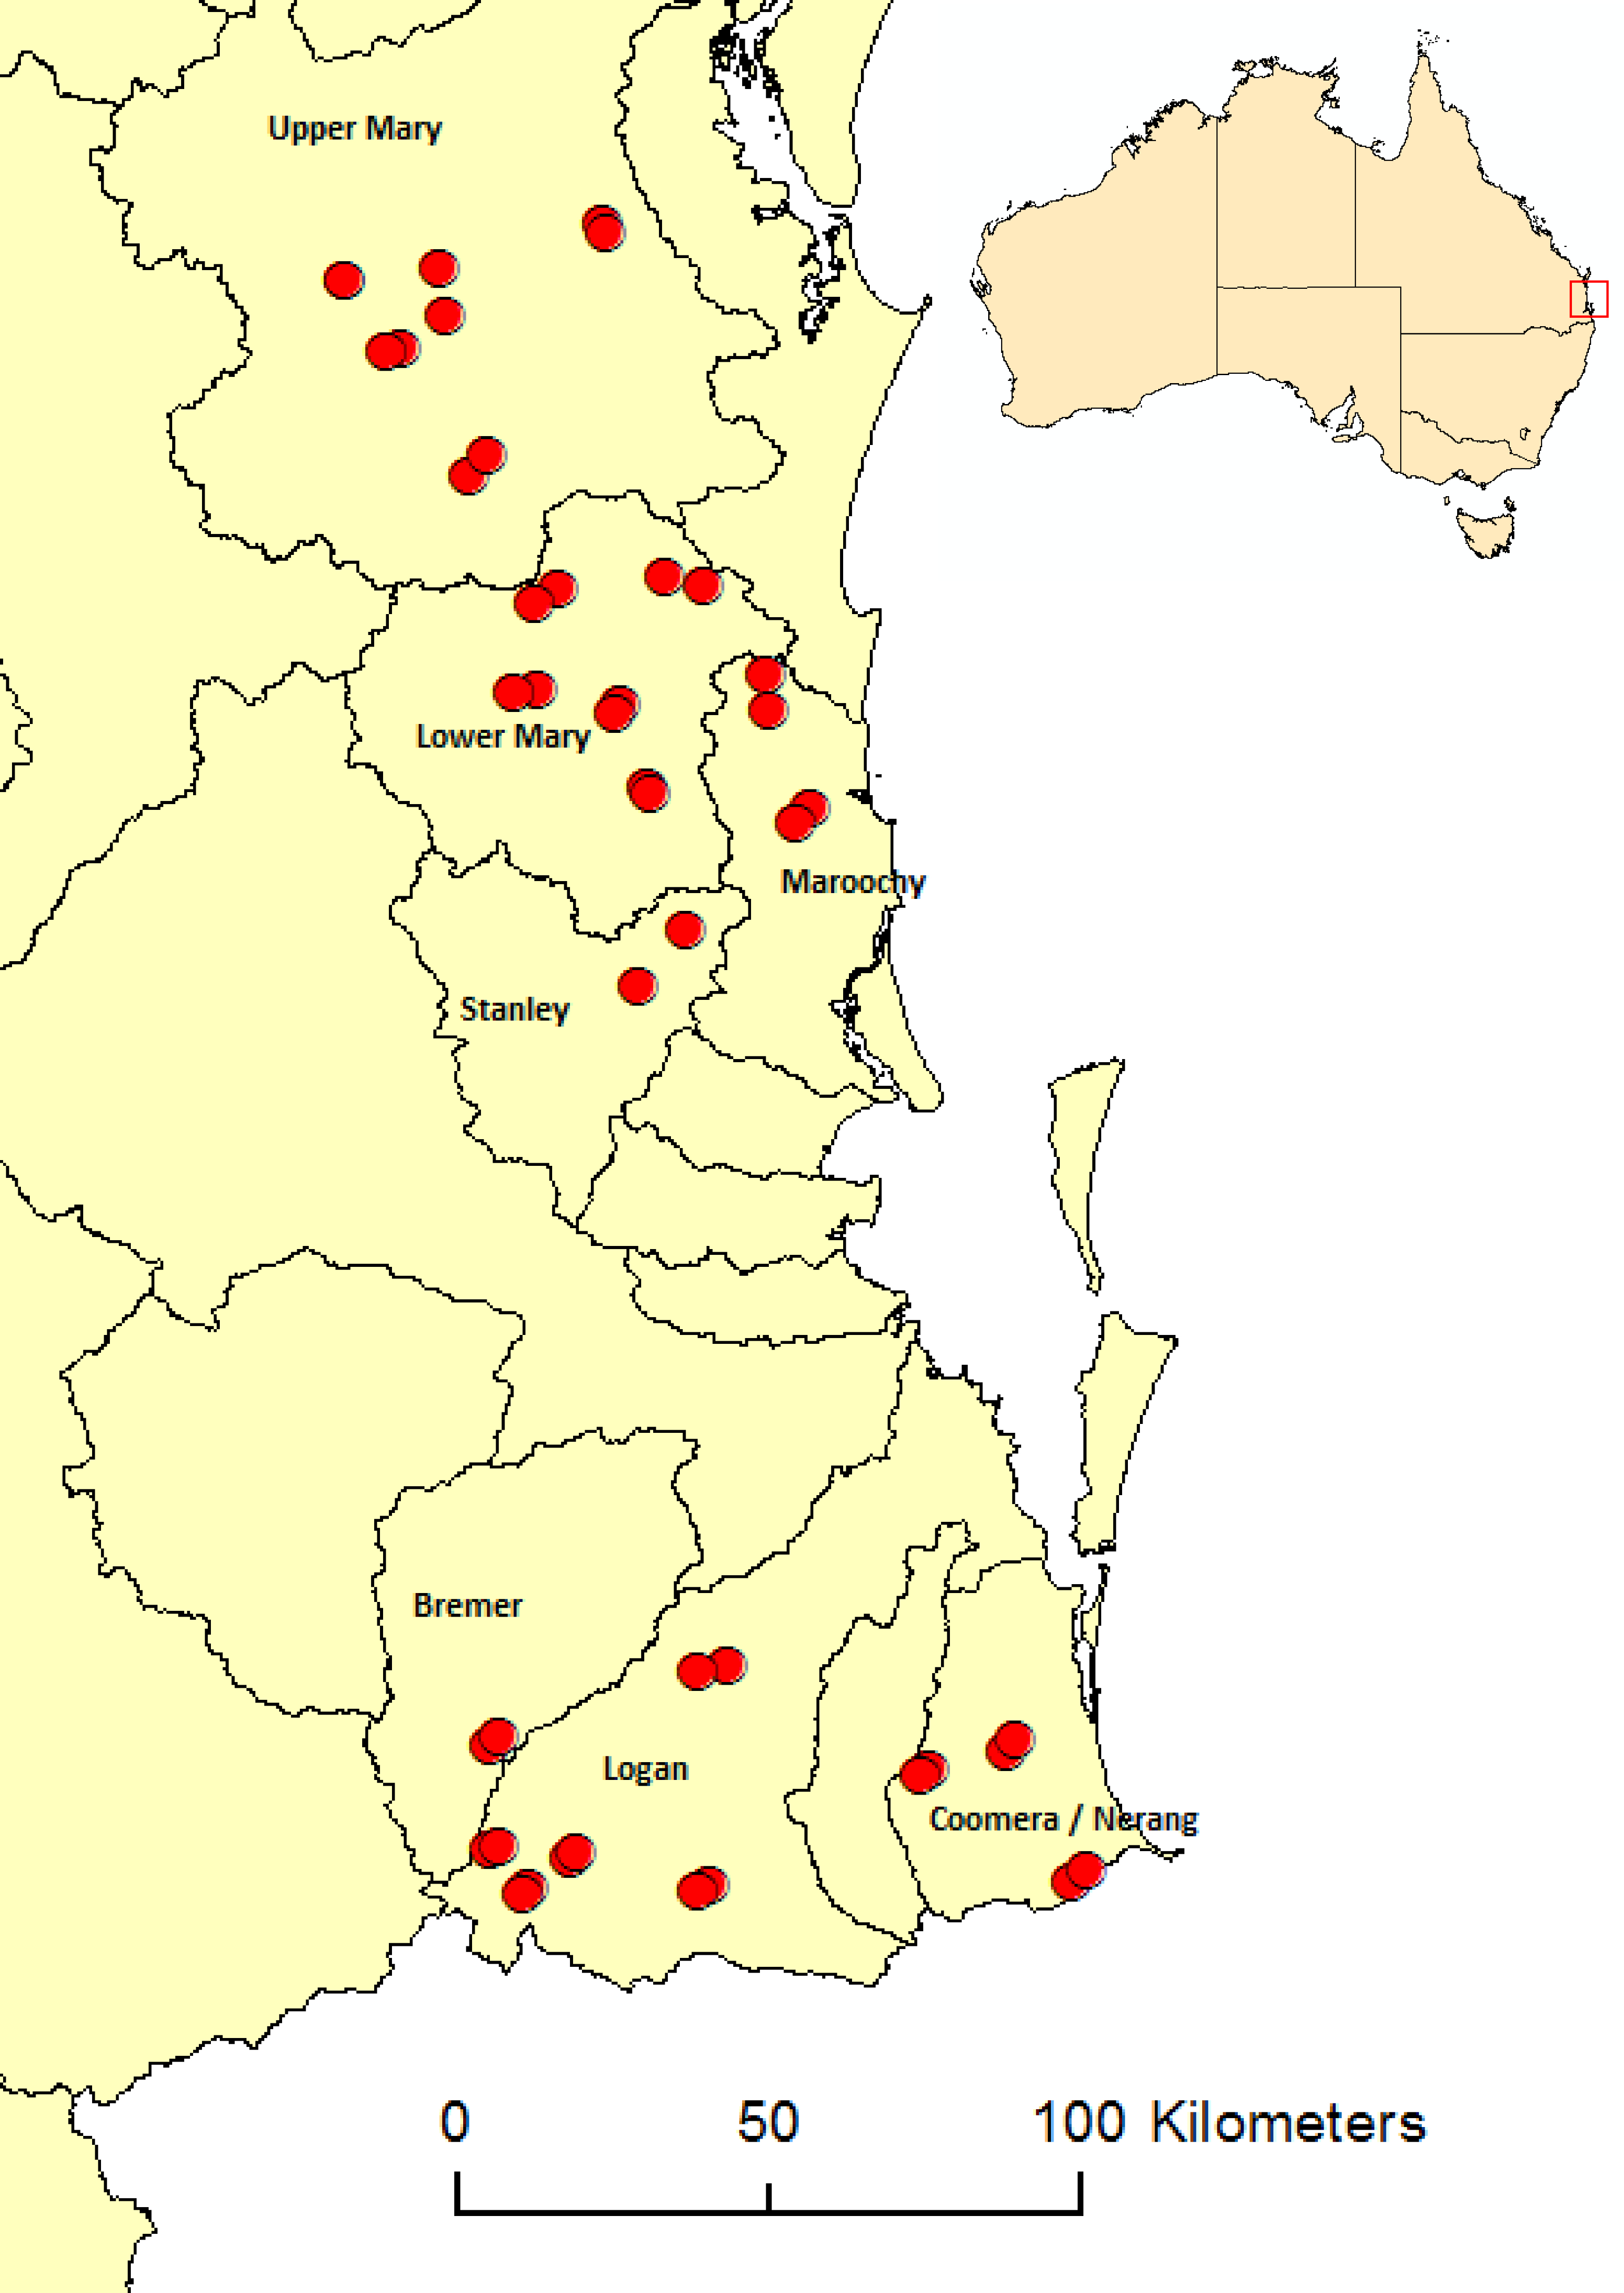
\includegraphics[width=12cm,keepaspectratio=true]{Ch4map2.png} % figures can be in pdf, png, jpeg or eps format
\caption[Study catchments and locations of field sites in south-eastern Queensland.]{\small{Study area (inset), study catchments and locations of field sites in south-eastern Queensland.}} %The caption in the square bracket is used for the table of figures. The caption in the curved brackets is the one that is printed as actual caption. 
\label{fig:Ch4_F1} % label for cross-referencing
\end{center}
\end{figure}   

\section{Methods}
The current study is an extension of a previous larger study \citep{Arthington2012}; the report describing the original study provides extensive detail not included here. Except where specified, all statistical analyses were performed using the R statistical programming environment \citep{RCoreTeam2015}, and statistical significance was thresholded at alpha $=$ 0.05.

\subsection{Site selection and vegetation sampling}
Riparian vegetation was surveyed between August and October in 2008, 2009 and 2010. Twenty river reaches were selected to sample the range of flow regime classes determined by a regional classification of flow regimes (see Mackay et al., 2014). Proximity to flow monitoring gauges with an associated recording history of $>$25 years was of primary importance. Duplicate surveys were made along each river reach as close as possible to the flow monitoring station (to give a total of 40 sites), but separated by at least 2 km. Sampling sites required 100 continuous metres of relatively intact riparian vegetation, which was not subjected to regular burning and had not been cleared in at least 20 - 30 years. Ideally sites were not currently grazed, although this restriction was relaxed somewhat given the extensive pastoral land use throughout the region. 

Three transects were randomly placed at each site, running perpendicular to the river. Additional transects were conducted at three sites, where low vegetation densities occurred. Transects extended from the water�s edge to the macrochannel bank, or to a maximum of 50 m from the water�s edge. A standard sampling area was not used due to variability in vegetation structure, channel landforms and adjacent land uses; sampling area was controlled for in subsequent analyses. Site sampling areas were typically greater than 400 m\textsuperscript{2} but ranged from 260 - 1013 m\textsuperscript{2}. All vascular plants within a 5 m band centred on the transect line were identified and counted. Species identifications were confirmed by the Queensland Herbarium. 

\subsection{Describing stream hydrology and quantifying flow regulation}
Daily discharge data for each reach were obtained from Queensland Government Department of Natural Resources and Mines (DNRM) Water Monitoring Data Portal \sloppy{\url{(https://www.dnrm.qld.gov.au/water/water-monitoring-and-data/portal)}}. 35 year time series spanning 1975 � 2009 were obtained where possible. Missing data were infilled using the Time Series Manager module in River Analysis Package \citep{marsh2003river}, using linear interpolation for periods less than 15 days, or multiple regression using data from adjacent stream gauges. One site (Reynolds Creek) had substantial periods of missing data which could not be infilled by multiple regression, as the flow at this gauge is altered by Moogerah Dam. The record for this site was truncated to exclude the periods where data was missing. The shortest remaining period (34 days) was infilled by linear interpolation. Flow data for one site (Obi Obi Creek at Kidaman) was obtained from Water Quality Accounting (Queensland DNRM) as modelled gauge data derived from a calibration model for the Mary River catchment. See \citet{Mackay2014} for further information on interpolation of hydrological data.

River Analysis Package was used to generate a set of 18 ecologically relevant hydrological metrics for each site, describing mean and interannual variability in the frequency, magnitude and duration and seasonal timing of high and low flow conditions. Table \ref{tab:Ch4_T1} provides definitions of these flow regime characteristics and describes their ecological importance and contribution to environmental heterogeneity. As a number of these metrics exhibited collinearity, we have included a principal components analysis of this data in Appendix 3a. Metrics of flow magnitude which had units ML / day were standardised by mean daily flow to allow for comparison between different river channel sizes. These metrics therefore represent ratios of flow magnitude to mean daily flow.

The extent of flow regulation at a given gauge site was characterised by the percentage deviation of each metric from the same metric generated using modelled pre-development flow data. These modelled pre-development daily discharge data were obtained from a generic integrated water quantity and quality simulation model (IQQM) developed for the region \citep{simons1996iqqm}. IQQM data were available only for the period up to 1999, so data from the timeframe 1975-1999 were used for comparison.


\begin{landscape}
\begin{tiny}
{\tabulinesep=1.2mm
\begin{longtabu} to \linewidth {m{6.5cm}m{2cm}m{2.2cm}X} 
\caption[Description of hydrological variables.]{Hydrological variables used as metrics of fluvially induced environmental heterogeneity in the riparian zone (adapted from \citep{Lawson2015a})}
\label{tab:Ch4_T1} \\
\hline
% -----------------These are headings----------------------------------%
\textit{Variable} & \textit{Abbreviation} & \textit{Units} & \textit{Description} \\ 
%
\endfirsthead
%
%\multicolumn{4}{c}%
%{{\bfseries  Continued from previous page}} \\
%\hline
%
\hline
\textit{Variable} & \textit{Abbreviation} & \textit{Units} & \textit{Description} \\ \hline
\endhead
%
%\hline \multicolumn{4}{|r|}{{Continued on next page}} \\ \hline
%\endfoot
%
%\hline
%\multicolumn{4}{|r|}{{Concluded}} \\ \hline
%\endlastfoot
%-----------Headings end---------------------------------
\hline
\multicolumn{4}{l}{\textbf{Frequency, magnitude and duration of floods and dry spells}} \\
Mean magnitude of high spells * & HSPeak & dimensionless & \multirow{12}{*}{\parbox{8.4cm}{Together, these metrics characterise the frequency, magnitude and duration of floods and dry spells. Extreme low or high flows contribute to spatial environmental heterogeneity, in that their effects (flooding disturbance, soil moisture stress) are spatially variable throughout the riparian landscape. High flow spells are periods of flow above the 95th percentile; low flow spells are periods of flow below the 5th percentile. \newline
HSPeak and LSPeak describes the mean magnitude of highest and lowest flows during high and low spells throughout the record, respectively. MDFAnnHSNum and MDFAnnLSNum describe the mean annual frequency of high and low spells. HSMeanDur and LSMeanDur describe how long flow events last. \newline
Coefficients of variation (CV) of these metrics between years characterise temporal heterogeneity in flow patterns.}} \\
Mean magnitude of low spells * & LSPeak & dimensionless &  \\
CV of all years' mean high spell magnitude & CVAnnHSPeak & dimensionless &  \\
CV of all years 'mean low spell magnitude & CVAnnLSPeak & dimensionless &  \\
Mean of all years' number of high spells & MDFAnnHSNum & year\textsuperscript{-1} &  \\
Mean of all years' number of low spells & MDFAnnLSNum & year\textsuperscript{-1} &  \\
CV of all years' number of high spells & CVAnnHSNum & dimensionless &  \\
CV of all years' number of low spells & CVAnnLSNum & dimensionless &  \\
High spell mean duration & HSMeanDur & days &  \\
Low spell mean duration & LSMeanDur & days &  \\
CV of all years' high spell mean duration & HSMeanDur & dimensionless &  \\
CV of all years' low spell mean duration & LSMeanDur & dimensionless &  \\
\tabularnewline
\hline
\newpage
\multicolumn{4}{l}{\textbf{Baseflow index}} \\
Baseflow index & BFI & dimensionless & \multirow{4}{*}{\parbox{8.4cm}{Baseflow index is calculated using the ratio of flow during average conditions to total flow. It is a useful metric of perenniality of water availability, in that it is maximised when average flow conditions dominate, and minimised when total flow is dominated by above average flow events. Thus higher baseflow systems experience more homogeneous flows.}} \\
CV of all year's baseflow index & CVAnnBFI & dimensionless &  \\[0.4cm]
& & & & \\
%\tabularnewline
\hline
%\newpage
\multicolumn{4}{l}{\textbf{Colwell's indices}} \\
Constancy of monthly minimum daily flow & C\_MinM & dimensionless & \multirow{4}{*}{\parbox{8.4cm}{Colwell's indices provide a measure of the seasonal predictability of flow events, and as such are a direct measure of temporal heterogeneity of flow patterns. \newline
Constancy (C) measures uniformity of flow across seasons, and is maximised when flow conditions do not differ between seasons. Contingency (M) is a measure of interannual uniformity in seasonal flow patterns, and is maximized when seasonal patterns of flow are consistent between years.  We generated Colwell's indices for both minimum and maximum flows conditions.}} \\
Contingency of monthly minimum daily flow & M\_MinM & dimensionless &  \\
Constancy based on monthly maximum daily flow & C\_MaxM & dimensionless &  \\
Contingency based on monthly maximum daily flow & M\_MaxM & dimensionless &  \\[0.5cm]
& & & & \\
\hline
%\newpage
\multicolumn{4}{l}{\textbf{Flow seasonality}} \\
Average mean daily dry season flow * & MDFMDFDry & dimensionless & \multirow{1}{*}{\parbox{8.4cm}{These metrics describe the average magnitude and temporal variability in mean daily flows for each season (dry = May to October, wet = November to April). Averages and coefficients of variation are calculated across yearly means. Seasonal average mean daily flows were standardised by overall mean daily flow, so actually represent the ratio of mean daily flow in a given season to the total mean daily flow.}} \\
Average mean daily wet season flow * & MDFMDFWet & dimensionless &  \\
CV of mean daily dry season flow & CVMDFDry & dimensionless &  \\
CV of mean daily dry season flow & CVMDFWet & dimensionless & \\[0.2cm] \\
\hline
\end{longtabu}}
\end{landscape}

\subsection{Other environmental variables}
Data on upstream land use were obtained via the Queensland Land Use Mapping Program (QLUMP) and dataset \citep{witte2006mapping}. These data were generated from surveys conducted in 1999 and 2006. Land use was categorised according to the Australian Land use and Management Classification version 6 \citep{BRS2002}, which differentiates conservation and low impact land uses from intensive land uses. Percentages of upstream land use were calculated as: production from relatively natural environments (forestry, grazing natural vegetation), dryland agriculture and plantations (e.g. cropping, horticulture, grazing pasture), irrigated agriculture (e.g. irrigated cropping, horticulture), conservation and natural environments (e.g. national park) and intensive uses (e.g. residential and industrial uses). We then used inverse distance weighting to weight each land use according to its proximity to the stream, following Petersen et al. (2010). 

Climate data were obtained from eMast/TERN, at a resolution of 0.01 degrees \citep{Hutchinson2014}. Bioclimatic variables representing annual trends, seasonality and extremes were calculated following the BIOCLIM framework \citep{busby1991bioclim}. The resulting set of 19 climate variables were strongly collinear, consequently PCA was used to identify a subset of six variables which represented over 90 \% of the variation in the data. Soil data were obtained from the CSIRO Soil and Landscape Grid of Australia, at a resolution of 3 arc seconds ({\raise.17ex\hbox{$\scriptstyle\mathtt{\sim}$}} 3 m) \citep{Rossel2014, Rossel2014a, Rossel2014b, Rossel2014c, Rossel2014d, Rossel2014e, Rossel2014f, Rossel2014g, Rossel2014h, Rossel2014i, Rossel2014j, Wilford2014}.

\subsection{Trait selection and dataset assembly}
We assembled a dataset of six continuous (specific leaf area, leaf area, maximum canopy height, seed mass, wood density and flowering duration) and one categorical (growth form) functional traits with which to calculate functional diversity. These traits collectively describe central trade-offs associated with ecological strategies of riparian plants (functional responses), as well as flow-on effects of species on ecosystem functioning (functional effects). Table \ref{tab:Ch4_T2} provides further description of the utility of each of these traits in characterising the functional ecology of riparian vegetation communities.

Data was taken from published literature, private and published trait datasets, and Australian flora texts. Substantial contributions were taken from the following sources: \citep{KEWseed, plantnet, zanne2009global, Wright2000, Fonseca2000, Gallagher2012a, Kooyman2013, Gleason2012} as well as from Ian Wright (pers. comm.) and Cassandra James (pers. comm.). Where multiple records for a trait were found, values were removed if they were measured at sites with an environment substantially different from south east Queensland. With the exception of maximum height, for which the highest value was used, the remaining values were averaged to provide a single value for each species-trait combination. Not all species-trait combinations could be assigned data, so to reduce biases associated with analyses of incomplete trait datasets \citep{Penone2014}, only species with fewer than 3 missing trait values (174 / 260) were retained for the analysis. The remaining missing values were imputed using a non-parametric random forests approach (missForest package for R) \citep{Stekhoven2012}. Dataset density information and imputation error estimates can be found in Appendix 3a.

\begin{landscape}
\begin{tiny}
{\tabulinesep=1.2mm
\begin{longtabu} to \linewidth {lp{5cm}XX} 
\caption[Traits included in functional diversity analysis.]{Rationale for selection of functional response and effect traits as descriptors of riparian plant community functional diversity.}
\label{tab:Ch4_T2} \\
\hline
% -----------------These are headings----------------------------------%
\textit{Trait} & \textit{Definition} & \textit{Functional responses} \& \textit{inherent trade-offs} & \textit{Functional effects} \\ 
%
\endfirsthead
\hline
\textit{Trait} & \textit{Definition} & \textit{Functional responses} \& \textit{inherent trade-offs} & \textit{Functional effects} \\  \hline
\endhead
\hline
Growth form & Categorical description of morphology: tree, shrub, woody climber, herbaceous climber, graminoid, herb. & Differential responses to mechanical and biochemical stresses associated with flooding; different strategies for coping with drought and heat stress. & Differential biogeomorphic effects on surface roughness, sediment deposition and fluvial landform cohesion. \\
Specific leaf area (SLA) & Ratio of one-sided leaf area to oven dry mass (cm\textsuperscript{2} / g). & SLA is associated with leaf construction cost, photosynthetic rate and carbon : nitrogen economics. Indicator of  ecological strategy under favourable vs. stressful conditions \citep{Wright2004}. & Affects ecosystem productivity and nutrient recycling \citep{Wright2004}. \\
Leaf area & One-sided leaf area (cm\textsuperscript{2}). & Shade tolerance (larger leaves) vs. enhanced thermal regulation ability in hot, dry conditions (smaller leaves) \citep{Cornelissen2003}. & May influence flow resistance of vegetation (and therefore fluvial erosion / deposition) when inundated. \\
Maximum canopy height & Height above ground of apical meristem (m). & Affects ability to tolerate mechanical disturbances such as flooding and maintain xylem integrity in dry conditions \citep{Westoby2006}. & Determines coarse physical structure of plant community. Surrogate for competitive ability: taller plants receive more light but must construct and maintain support structures \citep{Falster2006}. \\ \hline
Seed mass & Combined mass of the seed coat, endosperm and embryo (g). Excludes dispersal structures. & Larger seed mass confers ability to establish in unfavourable conditions \citep{Leishman2000}. Also related to seed buoyancy \citep{Carthey2015}. & Seeds may be an important food source for animals. \\
Wood density & Oven dry mass divided by green volume (g / cm\textsuperscript{3}) & Dense wood tissue confers mechanical strength, but is energetically expensive to construct. Wood density influences ability to tolerate drought stress and disturbance \citep{telewski1995wind, Preston2006, Lawson2015}. & Regulates decomposition rate; this affects nutrient cycling and determines the residency time of woody debris in the fluvial system \cite{mackensen2003decomposition}. \\
Flowering period length & Proportion of the year spent in flower (proportion, dimensionless). & Indicates species ability to respond reproductively to favourable conditions. & Flowers may be an important food source for animals. \\ \hline
\end{longtabu}}
\end{tiny}
\end{landscape}


\subsection{Calculating functional diversity, species richness and proportional abundance of exotics}
Functional richness (FRic) and functional divergence (FDiv) are complementary metrics of functional trait diversity, which together, describe the range and distribution of trait values in a community \citep{Villeger2008}. Functional evenness is also included in the framework introduced by Vill�ger et al. (2008) but has since shown limited ability to describe change in functional composition across environmental gradients \citep{Pavoine2011, Mason2012}. FRic represents the volume of the convex hull of trait values in a given community while FDiv provides information about the abundance distribution of trait values across this range.

We calculated functional richness and abundance-weighted functional dispersion (FDis) of vegetation communities at each site, using the FD package for R \citep{Laliberte2010}. Gower�s method, which scales traits by their range, was used to generate the required dissimilarity matrix, and Cailliez�s correction was applied to allow for PCoA axes corresponding to negative eigenvalues and render the matrix Euclidean \citep{Cailliez1983}. We transformed FRic and FDis into standardised effect sizes (SES): SES $=$ (obs - nullExp) / sd(nullExp), where obs is the observed functional diversity value and nullExp and sd(nullExp) are the mean and standard deviation of the expected functional diversity in 999 randomized communities \citep{Gotelli2002}. The null model for comparison with FRic was generated using the trial-swap algorithm \citep{Miklos2004} in the picante package \citep{kembel2010picante} to remove dependence on species richness. The null model for comparison with FDis was generated by randomizing abundances among species but within plots (using the resamp.2s  function in spacodiR) \citep{eastman2011spacodir}, to generate a metric of pure functional divergence (FDiv). The resulting indices, FRic.SES and FDis.SES, have greater power to detect community assembly processes than their unstandardised counterparts or the metric of functional divergence defined by Vill�ger et al. (2008) \citep{Mason2013}.

To more closely comply with the assumptions of statistical tests, trait values were normalised by either log\textsubscript{10} (SLA, seed mass) or square root (leaf area, maximum height, flowering duration) transformation prior to analysis. Wood density was not transformed. Summary statistics for the trait dataset are shown in Appendix 3a.

True species richness values were estimated by rarefaction according to species accumulation across the three replicate transects taken at each site. We used the "chao1" function in the fossil package in R \citep{vavrek2011fossil} to calculate abundance-based Chao's Species Estimator \citep{chao1987}. Abundance of exotic species was calculated as the number of exotic individuals divided by the total number of individuals counted at each site.

\subsection{Constructing variance partitioning models}
We used a variance partitioning approach to assess the individual contributions of river flow regime, flow modification, land use, climate and soil properties to modelling variation in riparian plant species richness, functional diversity and exotic abundance. Exotic proportional abundance was also included as an explanatory variable for species richness and functional diversity metrics. 

The following process was used to derive an optimal set of environment-diversity models for variance partitioning analysis \citep{Legendre2007}:
We first generated minimal multiple regression models for each set of environmental variables (i.e. descriptors of flow regime, flow modification, land use etc.): for each individual dependent variable, the full set of explanatory variables was reduced to the subset which showed statistically significant (p $<$ 0.05) linear or quadratic relationships. Second order AIC was used to determine whether the linear or quadratic term better explained variation in the dependent variable (MuMIn package for R) \citep{barton2012mumin, burnham2002model}. For each set of environmental variables, variance explained by significant univariate models was partitioned by partial regression using the varpart function in R (vegan package) \citep{Oksanen2013}. Multiple regression models were derived from the combinations of variables with the highest adjusted R\textsuperscript{2} values \citep{Peres-Neto2006}. These multiple regression models optimally combine the variation explained by all significant univariate models.

The four best multiple regression models were fed into a second variance partitioning analysis, and adjusted R\textsuperscript{2} was used to estimate the proportion of variation jointly and independently explained by each environmental model.  

\section{Results}
Below we describe the patterns of variation in species richness, exotic abundance, functional richness and functional dispersion of riparian plant communities, as they relate to metrics describing river hydrology, flow modification, land use, climate and soil properties.  
Due to considerable collinearity in the environmental dataset, description of univariate relationships is generally limited here to variables selected by variance partitioning for inclusion in the final multiple regression models. Statistics for the all statistically significant univariate regression models can be found in Appendix 3b. The adj. R\textsuperscript{2} value shown in variance partitioning Venn diagrams (Figs \ref{fig:Ch4_F2}-\ref{fig:Ch4_F5}b) may not correspond directly to the sum of its fractions as represented in Figs \ref{fig:Ch4_F2}-\ref{fig:Ch4_F5}a., as negative R\textsuperscript{2} values (not shown in Figs \ref{fig:Ch4_F2}-\ref{fig:Ch4_F5}a) can result from the adjustment algorithm. All R\textsuperscript{2} values given in the text are adjusted R\textsuperscript{2}. 

\subsection{Environmental drivers of variation in species richness}
The majority of variation in species richness across the study area (0.635) could be explained by a combination of models describing flow modification, climate and soil conditions (Fig. \ref{fig:Ch4_F2}a,b). The hydrological model explained no variation in species richness independently. There was no significant relationship between total species richness per hectare and exotic species richness per hectare, and although species richness did decrease with exotic proportional abundance (R\textsuperscript{2}  $=$ 0.152) (see Appendix 3b), exotic abundance did not independently explain variation in species richness.

A weak but significant model associated richer plant communities with sites which experienced unevenly distributed patterns of minimum flows (C\_MinM, R\textsuperscript{2}  $=$ 0.098, Fig. \ref{fig:Ch4_F2}c), and where those patterns tended to be consistent between years (M\_MinM, R\textsuperscript{2}  $=$ 0.130, Fig. \ref{fig:Ch4_F2}d). Greater interannual consistency in patterns of maximum flows was also associated with richer communities (M\_MaxM, R\textsuperscript{2}  $=$ 0.207, Fig. \ref{fig:Ch4_F2}e), although a pair of sites caused the quadratic model to dip at the upper bounds of consistency. Variation in species richness was well explained by modification of seasonal consistency of minimum flow patterns (M\_MinM.mod, R\textsuperscript{2}  $=$ 0.342, Fig. \ref{fig:Ch4_F2}f), despite the relatively weak relationship between species richness and M\_MinM. A significant quadratic relationship was found between species richness and modification of seasonal consistency of maximum flow conditions (M\_MaxM.mod, R\textsuperscript{2}  $=$ 0.243, Fig. \ref{fig:Ch4_F2}g); in this case the relationship was corroborated by a similar distribution over M\_MaxM. Species richness declined with increasing interannual variability in baseflow index (CVAnnBFI.mod, R\textsuperscript{2}  $=$ 0.108, Fig. \ref{fig:Ch4_F2}h). With respect to climate, species richness was greater at sites which experienced higher rainfall in both dry (clim\_pdry, R\textsuperscript{2}  $=$ 0.417, Fig. \ref{fig:Ch4_F2}i) and wet seasons (clim\_pwet, R\textsuperscript{2}  $=$ 0.465, Fig. \ref{fig:Ch4_F2}j), and declined as temperature seasonality increased (clim\_tsea, R\textsuperscript{2}  $=$ 0.349, Fig. \ref{fig:Ch4_F2}k). Lower soil cation exchange capacity (soil\_ece, R\textsuperscript{2}  $=$ 0.373, Fig. \ref{fig:Ch4_F2}l) and soil organic carbon content (soil\_soc, R\textsuperscript{2}  $=$ 0.252, Fig. \ref{fig:Ch4_F2}l) also were associated with richer communities.

The data did not support hypothesis 1, that rivers with more heterogeneous flow regimes support communities with higher species richness. In fact, greater species richness at sites which experienced less variabilty in timing of minimum flow patterns (Fig. \ref{fig:Ch4_F2}d) supports the counter-argument - species richness here is associated with less flow heterogeneity. Hypothesis 2, that there is a unimodal relationship between species richness and flow heterogeneity, was supported by a single relationship (M\_MaxM, Fig. \ref{fig:Ch4_F2}e), although the effect of modification of M\_MaxM towards less flow heterogeneity was also strongly unimodal (M\_MaxM.mod, Fig. \ref{fig:Ch4_F2}g). These results also contradict hypothesis 4 (that species richness and functional diversity should decrease along gradients of increasing flow modification and catchment land-use intensity), given that rivers with artificially increased consistency of minimum flow patterns (M\_MinM.mod, Fig. \ref{fig:Ch4_F2}f) and lower interannual variability in baseflow index (CVAnnBFI.mod, Fig. \ref{fig:Ch4_F2}h) hosted richer plant communities.


\begin{landscape}
\begin{figure}[ht]
\centering
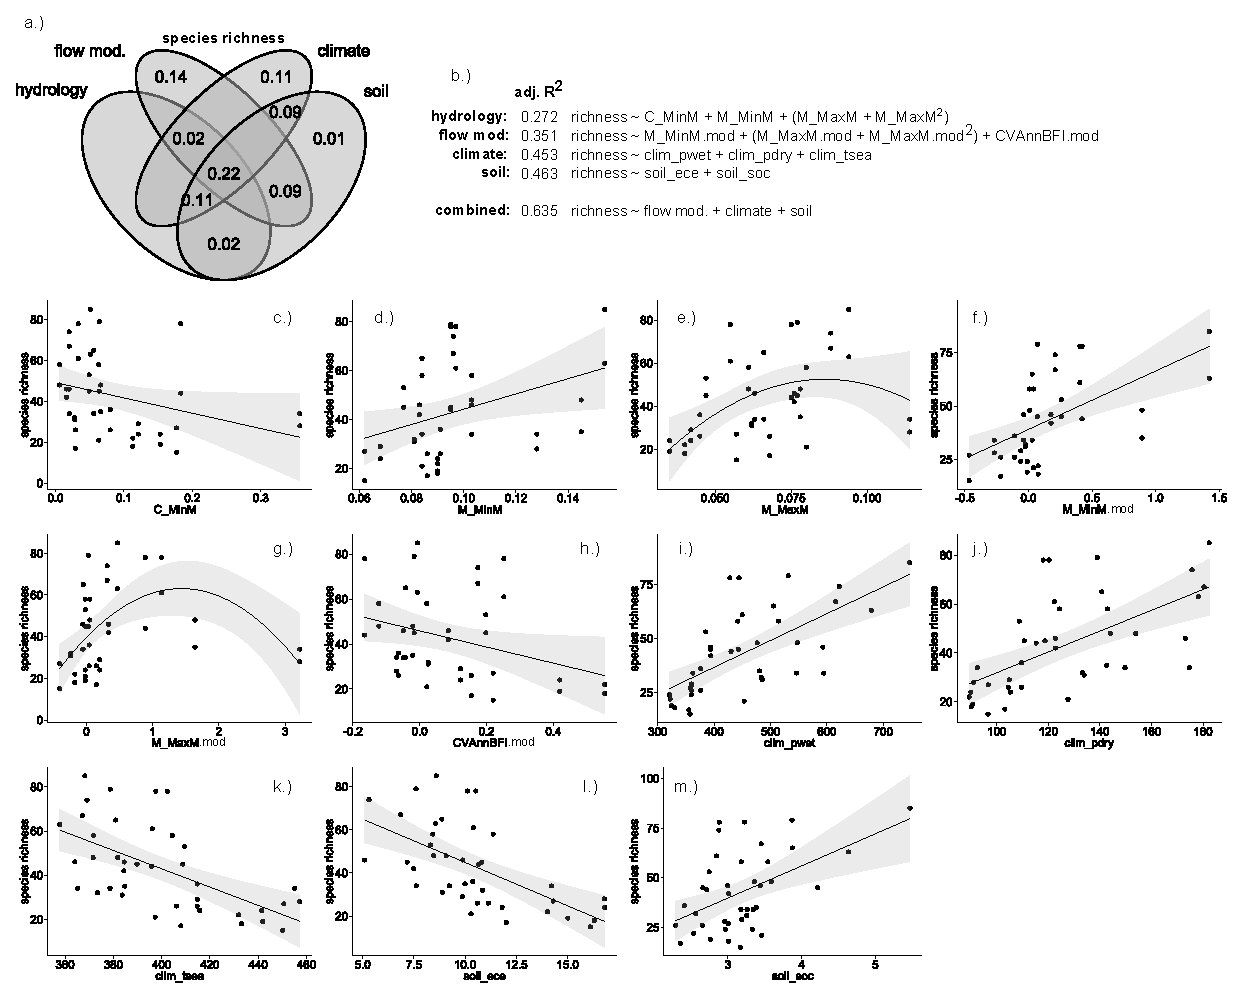
\includegraphics[height = \textheight]{Ch4speciesRichness_chao.pdf} % figures can be in pdf, png, jpeg or eps format
\end{figure}
\clearpage % insert a page break
\end{landscape}
\begingroup
\captionof{figure}[Environmental drivers of area-standardised species richness in riparian plant communities.]{\small{Environmental drivers of area-standardised species richness (units = species per m\textsuperscript{2}) in riparian plant communities. a.) variance partitioning Venn diagram. Numbers within the diagram represent adjusted R\textsuperscript{2}  (adj. R\textsuperscript{2}) values associated with each fraction of variation; b.) multiple regression models representing each set of environmental conditions, and their optimal combination. Quadratic terms are enclosed in parentheses. Selected univariate relationships between species richness and environmental variables describing c.) constancy of monthly minimum daily flows (C\_MinM); d.) contingency of monthly minimum daily flows (M\_MinM); e.) contingency of monthly maximum daily flows (M\_MaxM); f.) modification of contingency of monthly minimum daily flows (M\_MinM.mod, \% change); g.) modification of contingency of monthly maximum daily flows (M\_MaxM.mod, \% change); h.) modification of interannual variability in baseflow (CVAnnBFI);i.) precipitation in the wettest quarter of the year (clim\_pwet, mm); j.) precipitation in the driest quarter of the year (clim\_pdry, mm); k.) temperature seasonality (clim\_tsea) l.) soil effective cation exchange capacity (soil\_ece, meq per 100 g); m.) soil organic carbon content (soil\_soc, \%). Species richness is presented as the abundanced-based Chao's Species Estimator. Fitted lines depict ordinary least-squares regression models. Shaded areas depict the smoothed 95 \% confidence interval around the regression model.}}} 
\label{fig:Ch4_F2} % label for cross-referencing\endgroup
\clearpage

\subsection{Environmental drivers of functional richness (FRic.SES)}
Variation in FRic.SES was best explained by a combination of hydrological and soil models (variation explained by the combined model $=$ 0.405) (Fig. \ref{fig:Ch4_F3}a,b), of which the hydrological model gave the most explanatory power. Soil variables independently explained a small fraction of variation, and while flow modification and climatic variables were also associated with FRic.SES, neither model explained any variation independently. 

FRic.SES was distributed unimodally across gradients of interannual variability in baseflow index (CVAnnBFI, R\textsuperscript{2}  $=$ 0.170, Fig. \ref{fig:Ch4_F3}c); the modelled slope increased steeply at the lower end of the gradient but was only somewhat reduced from the peak by the top of the gradient. Greater frequency of high flow periods was associated with lower functional richness (MDFAnnHSNum, R\textsuperscript{2}  $=$ 0.142, Fig. \ref{fig:Ch4_F3}d). FRic.SES also declined as rainfall (clim\_pwet, R\textsuperscript{2}  $=$ 0.246, Fig. \ref{fig:Ch4_F3}e), soil total nitrogen (soil\_nto, R\textsuperscript{2}  $=$ 0.144, Fig. \ref{fig:Ch4_F3}f) and soil organic carbon (soil\_soc, R\textsuperscript{2}  $=$ 0.257, Fig. \ref{fig:Ch4_F3}g) increased. 

Hypothesis 1 was not supported, given that reduced functional richness was associated with increasing frequency of high flows. Hypothesis 3 was supported by a significant unimodal relationship interannual variability in baseflow (Fig. \ref{fig:Ch4_F3}c) and functional richness (delta AICc between linear and quadratic models $=$ 3.70). Although not selected for the final hydrological model, mean and interannual variability in duration of high flow periods (HSMeanDur, CVAnnHSMeanDur) also showed significant unimodal relationships with FRic.SES (R\textsuperscript{2}  $=$ 0.213, 0.182, respectively; Appendix 3b). Hypothesis 4 was not supported: we found no effect of either land use or flow modification on functional richness, except a weak relationship with modification of dry season mean daily flow (Appendix 3b). 

\begin{landscape}
\begin{figure}[ht]
\centering
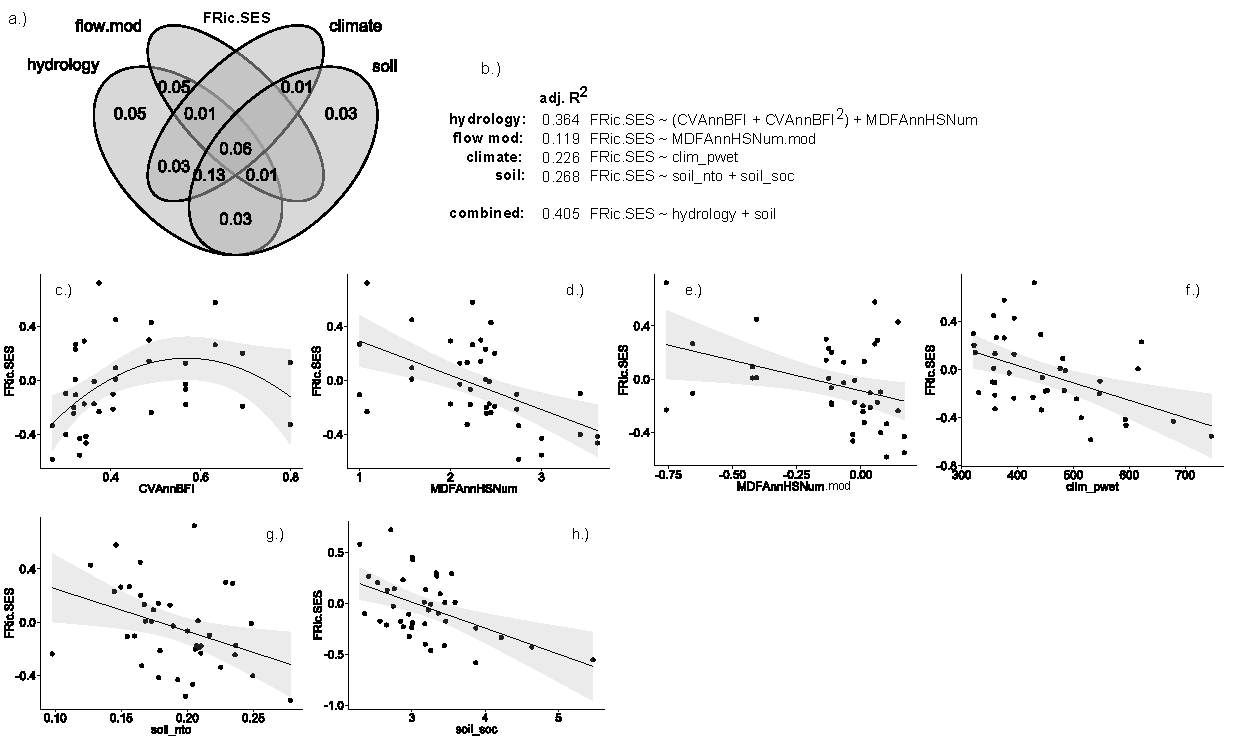
\includegraphics[height = \textheight]{Ch4FRicSES1.pdf} % figures can be in pdf, png, jpeg or eps format
\end{figure}
\clearpage % insert a page break
\end{landscape}
\begingroup
\captionof{figure}[Environmental drivers of standardised effect size functional richness (FRic.SES) in riparian plant communities.]{\small{Environmental drivers of standardised effect size functional richness (FRic.SES) in riparian plant communities. a.) variance partitioning Venn diagram. Numbers within the diagram represent adjusted R\textsuperscript{2}  (adj. R\textsuperscript{2} ) values associated with each fraction of variation; b.) multiple regression models representing each set of environmental conditions, and their optimal combination. Quadratic terms are enclosed in parentheses. Selected relationships between FRic.SES and environmental variables describing c.) interannual variability in baseflow (CVAnnBFI); d.) mean annual frequency of high flow periods (MDFAnnHSNum); e.) modification of mean annual frequency of high flow periods (MDFAnnHSNum.mod, \% change); f.) precipitation in the wettest quarter (clim\_pwet, mm); g.) soil total nitrogen (soil\_nto, \%); h.) soil organic carbon (soil\_soc, \%). Fitted lines depict ordinary least-squares regression models. Shaded areas depict the smoothed 95 \% confidence interval around the regression model.}}
\label{fig:Ch4_F3} % label for cross-referencing
\endgroup
\clearpage

\subsection{Environmental drivers of functional divergence (FDis.SES)}
FDis.SES varied substantially across the study area (3.96 standard deviations of the null distribution), and was associated with gradients of hydrology, flow modification, climatic and soil conditions. The soil model explained 0.483 of the variation in FDis.SES; hydrology, flow modification and climatic models did not independently explain further variation (Fig. \ref{fig:Ch4_F4}a,b). 

Rivers with moderate seasonality of maximum flows tended to support communities with high functional divergence (C\_MaxM, R\textsuperscript{2}  $=$ 0.321, Fig. \ref{fig:Ch4_F4}c). The entire range of FDis.SES was represented by rivers associated with highly seasonal patterns of maximum flows (C\_MaxM), however. As with functional richness, FDis.SES declined with increasing frequency of high flows (MDFAnnHSNum, R\textsuperscript{2}  $=$ 0.112, Fig. \ref{fig:Ch4_F4}d). Functional divergence also varied with flow modification affecting high flow frequency (MDFAnnHSNum.mod, R\textsuperscript{2}  $=$ 0.144, Fig. \ref{fig:Ch4_F4}e): lower flooding frequency tended to be associated with higher functional divergence. Also tracking trends observed for FRic.SES, FDis.SES declined with increasing rainfall (clim\_pwet, R\textsuperscript{2}  $=$ 0.141, Fig. \ref{fig:Ch4_F4}f), soil total nitrogen (soil\_nto, R\textsuperscript{2}  $=$ 0.111, Fig. \ref{fig:Ch4_F4}g) and soil organic carbon (soil\_soc, R\textsuperscript{2}  $=$ 0.344, Fig. \ref{fig:Ch4_F4}h).

Environmental heterogeneity (as indicated by high flow frequency) was associated with lower functional divergence (Fig. \ref{fig:Ch4_F4}d,e), opposing the prediction made in hypothesis 1, while the unimodal relationship with constancy of maximum flows (Fig. \ref{fig:Ch4_F4}c) provided some support for hypothesis 3 (delta AICc between linear and quadratic models $=$ 10.08). Scant evidence to support hypothesis 4 was found: as with FRic.SES, a weak but significant relationship was present between FDis.SES and modification of flood frequency (Fig. \ref{fig:Ch4_F4}d).

\begin{landscape}
\begin{figure}[ht]
\centering
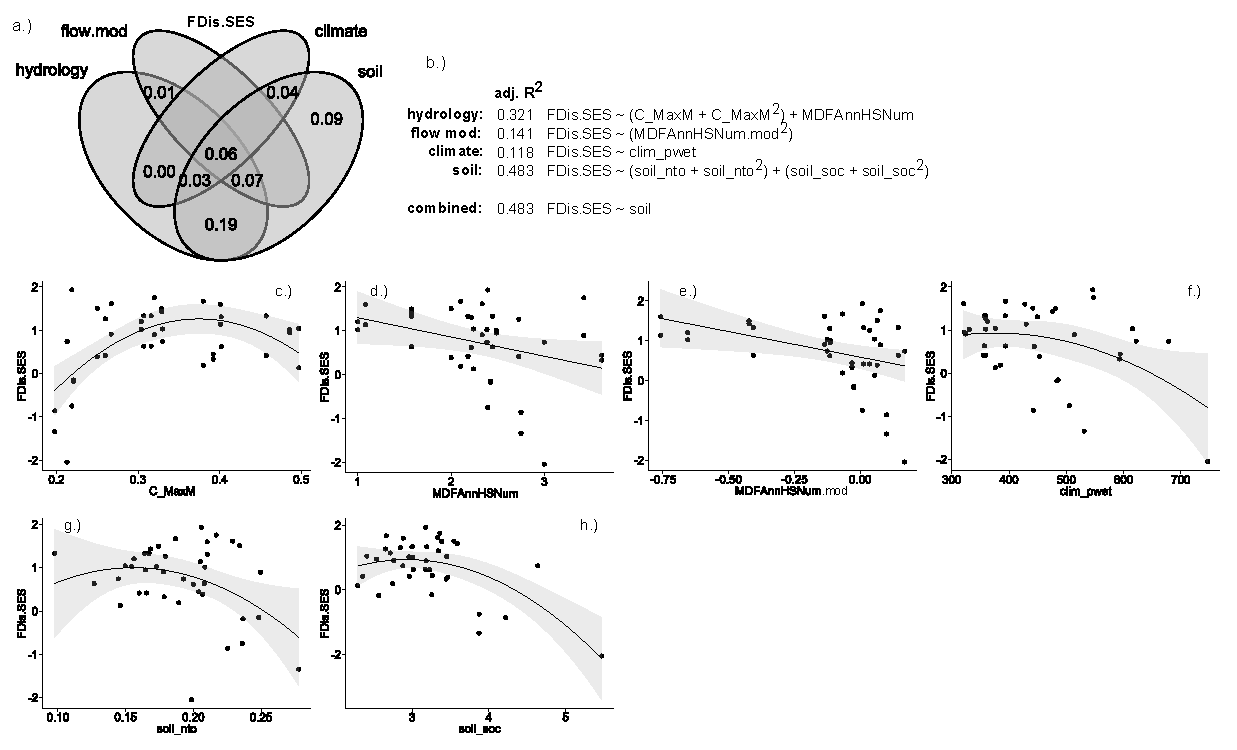
\includegraphics[height = \textheight]{Ch4FDisSES.pdf} % figures can be in pdf, png, jpeg or eps format
\end{figure}
\clearpage % insert a page break
\end{landscape}
\begingroup
\captionof{figure}[Environmental drivers of standardised effect size functional dispersion (FDis.SES) in riparian plant communities.]{\small{Environmental drivers of standardised effect size functional dispersion (FDis.SES) in riparian plant communities. a.) variance partitioning Venn diagram. Numbers within the diagram represent adjusted R\textsuperscript{2}  (adj. R\textsuperscript{2} ) values associated with each fraction of variation; b.) multiple regression models representing each set of environmental conditions, and their optimal combination. Quadratic terms are enclosed in parentheses. Selected relationships between FDis.SES and environmental variables describing c.) constancy of monthly maximum daily flows (C\_MaxM); d.) mean annual frequency of high flow periods (MDFAnnHSNum); e.) modification of mean annual frequency of high flow periods (MDFAnnHSNum.mod, \% change); f.) precipitation in wettest quarter (clim\_pwet, mm); g.) soil total nitrogen (soil\_nto, \%); h.) soil organic carbon (soil\_soc, \%). Fitted lines depict ordinary least-squares regression models. Shaded areas depict the smoothed 95 \% confidence interval around the regression model.}}
\label{fig:Ch4_F4} % label for cross-referencing
\endgroup
\clearpage

\subsection{Environmental drivers of variation in proportional abundance of exotic species}
Variation in exotic species abundance was jointly explained by hydrology, land use, soil and climatic models (0.665 of variation explained by the combined model) (Fig. \ref{fig:Ch4_F5}a,b). Hydrological models (0.581 of variation explained) and land use (0.515 of variation explained) models were dominant. Two individual metrics of flow modification had significant relationships with exotic abundance (C\_MinM.mod, R\textsuperscript{2}  $=$ 0.124; LSPeak.mod, quadratic R\textsuperscript{2}  $=$ 0.105), but these effects were strongly influenced by outlying values and the flow modification model combining these metrics explained no variation independently.

Exotic abundance closely tracked interannual variability in baseflow index (CVAnnBFI, R\textsuperscript{2}  $=$0.412, Fig. \ref{fig:Ch4_F5}c), and also rose as maximum flows became more uniformly distributed across seasons (i.e. a lack of flow seasonality) (C\_MaxM, R\textsuperscript{2}  $=$ 0.157, Fig. \ref{fig:Ch4_F5}d). We found a trough-shaped relationship between interannual variability in dry season flows and exotic abundance (CVMDFDry, R\textsuperscript{2}  $=$ 0.412, Fig. \ref{fig:Ch4_F5}e), although the lower end of the distribution was data-poor and may have been unduly influenced by values for a single pair of sites. Throughout the centre and upper ranges of the distribution, however, exotic abundance increased strongly with interannual variability in dry season flow. Exotic abundance also increased with interannual variability in high spell duration (CVAnnHSMeanDur, R\textsuperscript{2}  $=$ 0.129, Fig. \ref{fig:Ch4_F5}f). The proportion of the upstream catchment used for irrigated agricultural production was a strong positive predictor of exotic abundance (production\_irrigated, R\textsuperscript{2}  $=$ 0.37, Fig. \ref{fig:Ch4_F5}g), as was production from relatively natural environments, although somewhat less so (production\_natural, R\textsuperscript{2}  $=$ 0.232, Fig. \ref{fig:Ch4_F4}h). Exotic abundance declined as dry season precipitation increased (clim\_pdry, R\textsuperscript{2}  $=$ 0.207, Fig. \ref{fig:Ch4_F5}i), increased with soil pH (soil\_phc, R\textsuperscript{2}  $=$ 0.242, Fig. \ref{fig:Ch4_F5}j), and decreased with soil depth to hard rock (soil\_der, R\textsuperscript{2}  $=$ 0.140, Fig. \ref{fig:Ch4_F5}k).

With respect to hypothesis 2 (that abundance of exotic species should decline monotonically with increasing hydrological heterogeneity), we found the opposite of expected: hydrological heterogeneity (as measured by CVAnnBFI, CVMDFDry and CVAnnHSMeanDur) appears to be associated with higher exotic abundance. These relationships did not exhibit unimodality. Production land uses were associated with higher exotic abundance, supporting hypothesis 5 (that abundance of exotic species should increase along gradients of increasing flow modification and catchment land-use intensity).

\begin{landscape}
\begin{figure}[ht]
\centering
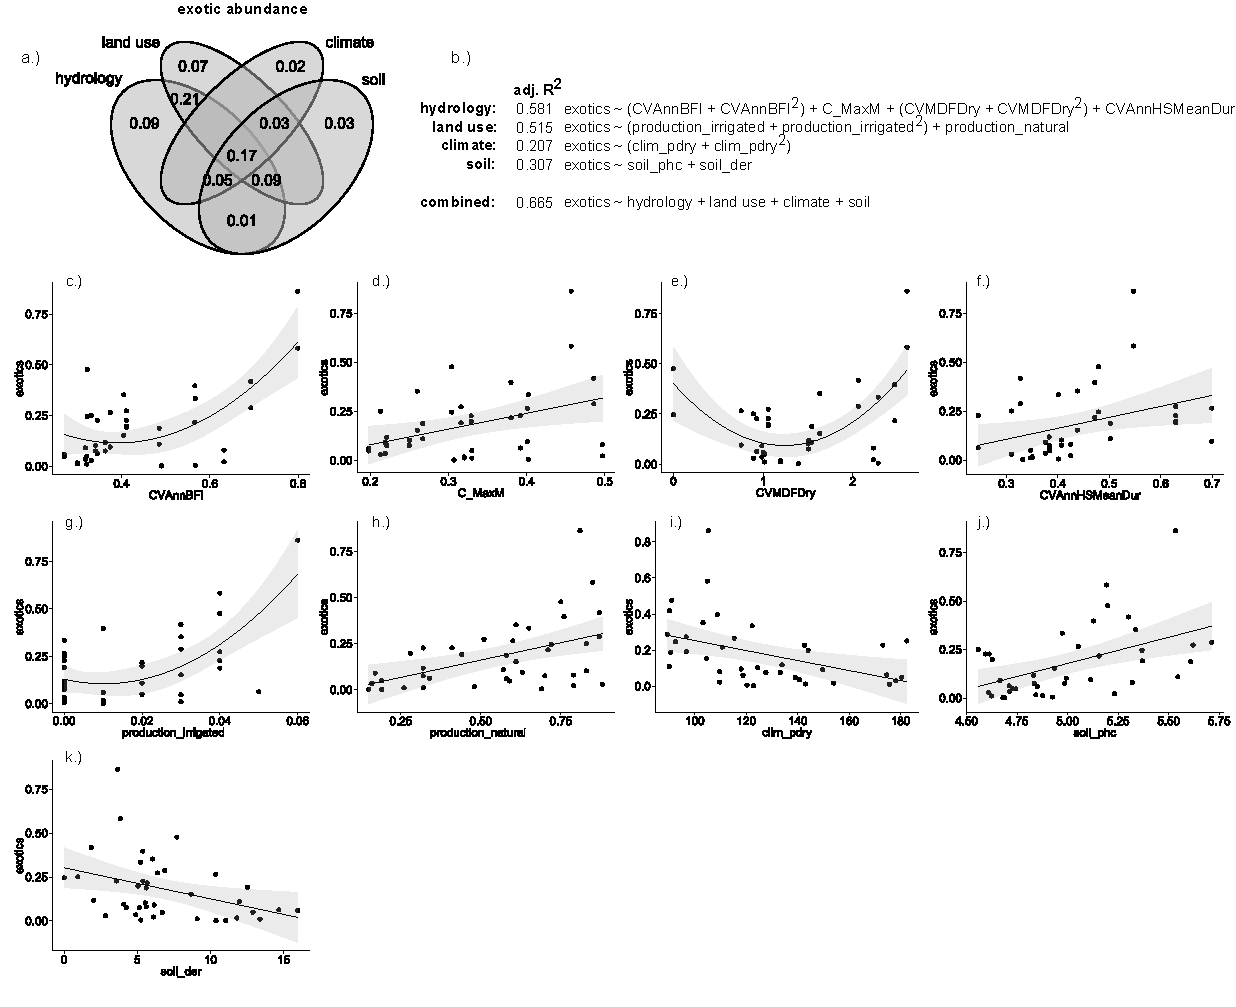
\includegraphics[height = \textheight]{Ch4exotics.pdf} % figures can be in pdf, png, jpeg or eps format
\end{figure}
\clearpage % insert a page break
\end{landscape}
\begingroup
\captionof{figure}[Environmental drivers of the proportional abundance of exotic species in riparian plant communities.]{\small{Environmental drivers of the proportional abundance of exotic species in riparian plant communities. a.) variance partitioning Venn diagram. Numbers within the diagram represent adjusted R\textsuperscript{2}  (adj. R\textsuperscript{2} ) values associated with each fraction of variation; b.) multiple regression models representing each set of environmental conditions, and their optimal combination. Quadratic terms are enclosed in parentheses. Selected relationships between exotic abundance and environmental variables describing c.) interannual variability in baseflow index (CVAnnBFI); d.) constancy of monthly maximum daily flows (C\_MaxM); e.) interannual variability in dry season mean daily flow (CVMDFDry); f.) interannual variability in mean duration of high flow periods; g.) proportion of catchment used for irrigated agricultural production (production\_irrigated, geographically weighted \%); h.) proportion of catchment used for production from relatively natural environments (production\_natural, geographically weighted \%); i.) precipitation in the driest quarter (clim\_pdry, mm); j.) soil pH (soil\_phc, \%); k.) depth of regolith (soil\_der, m to hard rock). Fitted lines depict ordinary least-squares regression models. Shaded areas depict the smoothed 95 \% confidence interval around the regression model.}}
\label{fig:Ch4_F5} % label for cross-referencing
\endgroup
\clearpage

\section{Discussion}
We proposed that generation of niche complexity by spatially and temporally heterogeneous environmental conditions is the dominant control on diversity in riparian plant communities. Under this framework, suppression of natural environmental heterogeneity by human modification of river flow regimes and catchment landscapes would result in lower diversity \citep{Poff1997, Poff2010}. This niche-oriented model of riparian plant diversity received mixed support in our study: by some metrics, species richness in fact decreased as hydrological conditions became more heterogeneous, and anthropogeneic flow homogenisation was associated with greater species richness. Although abundance of exotic species did increase with the proportion of surrounding land used for agricultural or silvicultural production, there was no relationship between exotic abundance and flow modification, and negative relationships were found with metrics of hydrological heterogeneity. The proportion of variation in functional diversity explained by environmental variables was comparatively lower than species richness or exotic abundance. Functional diversity metrics showed unimodal relationships with some metrics of hydrological heterogeneity, and declined with others. Flow modification was a weak predictor of functional diversity, and we found no effect of land use.

Given that a large proportion of variation in diversity metrics and exotic abundance explained by flow regime was co-explained by soil and climatic variables, is it possible to attribute flow regime as the dominant control on diversity? Taken individually, metrics of flow regime were the single best predictors of vegetation descriptors for FRic.SES (flood frequency, Fig. \ref{fig:Ch4_F3}d) and exotic abundance (interannual variability in dry season mean daily flows, Fig. \ref{fig:Ch4_F5}e). Species richness was best predicted by precipitation in the wet season (Fig. \ref{fig:Ch4_F2}i), while FDis.SES was best predicted by soil organic carbon content (Fig. \ref{fig:Ch4_F4}h). Variance partitioning showed that optimal models derived from flow regime metrics independently explained only a small proportion of variation in FRic.SES (Fig. \ref{fig:Ch4_F3}a)and exotic abundance (Fig. \ref{fig:Ch4_F5}a), and no independent variation in species richness (Fig. \ref{fig:Ch4_F2}a) or FDis.SES (Fig. \ref{fig:Ch4_F4}a). Extent of flow modification independently explained variation only in species richness, and changes to only a fraction hydrological metrics were important (Fig. \ref{fig:Ch4_F2}). 
As such it was not possible to give a conclusive affirmative response to this question; it is possible that relatively shallow extent of flow modification in the region over a relatively short timeframe ({\raise.17ex\hbox{$\scriptstyle\mathtt{\sim}$}}30 years) \citep{Mackay2014} did not provide the contrast required to find a consistent effect. The inherent dependency between between between climate and hydrology mean that manipulative experiments are required to confidently determine the influence of flow regime on riparian plant communities. 

Despite these limitations, we can make some interesting observations about the role of environmental heterogeneity as a driver of species richness in riparian plant communities. Contrary to expectation, sites with lower species richness were found where temporal patterns of minimum (Fig. \ref{fig:Ch4_F3}d) and maximum flows (Fig. \ref{fig:Ch4_F3}e) were less consistent between years, where interannual variability in baseflow was higher (Fig. \ref{fig:Ch4_F3}h), and also where temperature seasonality was greater (Fig. \ref{fig:Ch4_F3}k). A global meta-analysis of the ecology of tropical riverscapes showed that consistent, seasonal flow regimes support communities with higher net primary productivity and higher species richness in bird and fish assemblages than rivers with arrhythmic flow regimes \citep{Jardine2015}. Lundholm found in a meta-analysis of studies describing relationships between species richness, spatial environmental heterogeneity and energy availability, that energy availability was a better predictor of species richness than environmental heterogeneity \citep{Lundholm2009}. Temporal consistency in patterns of resource and energy availability may compete with environmental heterogeneity as a control on riparian plant diversity in this system. 

Further insight into the processes controlling riparian plant community assembly can be derived from patterns of functional diversity assembly across environmental gradients. FRic.SES represents the volume of the convex hull of trait values in a given community, as a fraction of the �expected� convex hull volume generated from randomized communities \citep{Mason2013}. FRic.SES is not weighted by species abundance and describes only the range of trait values present. FDis.SES, a pure measure of functional divergence \citep{Mason2013}, provides information about the abundance distribution of trait values across this range: functional divergence is maximised when highly abundant species are distant from the community centre of gravity in traitspace \citep{Mouchet2010}. Functional richness was unimodally related to temporal variability in baseflow index. The mechanism behind this is unclear, although following the line of reasoning developed for species richness, the effect of increased niche complexity may be offset by irregular resource availability and habitat microfragmentation as environmental heterogeneity increases \citep{Laanisto2013}.

Most communities had higher functional dispersion than predicted by the abundance-swapped null model, and a similar set of hydrological variables as FRic.SES had significant relationships with FDis.SES. FDis.SES showed a skewed, unimodal distribution across a gradient of constancy of maximum flows (C\_MaxM). Strongly negative values for several communities at the lower bound of C\_MaxM indicates functional underdispersion (i.e. environmental filtering), although the full range of variation in FDis.SES was present at low C\_MaxM \citep{Mason2013}. Variation in FDis.SES constricts as constancy increases, however, so with the exception of communities at this lower bound, communities along rivers with similar C\_MaxM tend to have similar species abundance distributions in traitspace. Interestingly, temporal variability in minimum flows (C\_MinM, M\_MinM) predicted species richness but temporal variability in maximum flows (C\_MaxM) predicted functional divergence. Compared with species richness, both FRic.SES and FDis.SES showed opposite relationships with climate and soil variables (clim_pwet, clim_tsea and soil_soc, among others), indicating that trait range is not reduced in concert with species richness. The traits which do remain are clustered towards the edges of the range, producing hollowed-out community trait distributions. 

Substantial variation in exotic abundance was jointly explained by hydrological and land use models. The proportion of catchment land-use associated with irrigated agricultural production was typically low, but production from natural environments (forestry etc.) was common and dominated a number of catchments. The rationale for our hypotheses was that environmental heterogeneity should result in structural complexity of habitat and therefore limit competitive exclusion by invasive species. We found that exotic abundance was associated with more hydrologically heterogeneous sites, and a greater proportion of catchment used for forestry. Thus the combined stresses of disturbance from forestry practices and heterogeneous flows may favour novel species assemblages. It is notable that flow modification was not significantly associated with exotic abundance, given that altered flow regimes have been linked to invasion in previous studies of regulated Australian river systems \citep{Catford2011, Greet2012a} (although see \citet{Merritt2010}). It may be significant that while these former studies found flow modification exacerbated invasion primarily by herbaceous species, the most dominant invaders in this study tended to be woody trees or vines (e.g. \textit{Leucaena leucocephala}, \textit{Macfadyena unguis-cati}, \textit{Celtis sinensis}).

Environmental conditions may also have interactive effects on exotic abundance and riparian plant diversity. We originally intended to model a set of competing hypotheses about the effects of interactions between environmental conditions on diversity and exotic abundance, but the analyses described here were performed post-hoc, and the scope of possible models proved too wide to winnow down based on our limited prior understanding of the system. Future studies which explicitly accommodate tests for interactions into experimental design may provide more insight into environmental controls on diversity.

Environmental models in this study accounted for only part of the total variation in functional diversity (40.5 \% for FRic.SES and 48.3 \% for FDis.SES). In a previous study of relatively unmodified riparian plant communities in south-eastern Australia, 80 \% of variation in functional dispersion was explained by a combination of variability in flood frequency, variability in flood magnitude, and mean daily summer flow \citep{Lawson2015a}. A fraction of this variation was independently explained by climate, and none was independently explained by soil variables. In contrast, much of the variance in functional diversity metrics in the current study was jointly explained by hydrological, climate and soil models. The weak link observed between functional diversity and flow modification (Fig. \ref{fig:Ch4_F3}e, Fig. \ref{fig:Ch4_F4}e) suggests that local land management practices and land use histories, which could not be accounted for in this study, may have had a strong influence on diversity \citep{Foster2003}. Additionally, our environmental gradient analyses are based on a niche optimisation paradigm of community assembly, and do not account for neutral processes or biotic interactions \citep{Kraft2015}. Competitive interactions may play a more important role in assembly of diverse subtropical plant communities than in more austere environments dominated by abiotic forces \citep{callaway1995positive}. Indeed, as is characteristic of subtropical forests, many of the species identified in this study were not obligate riparian species (James et al., in review) and could not necessarily be expected to display traits associated with adaptation to the riparian environment. 

Despite previous findings that ecosystem multifunctionality scales linearly with functional divergence \citep{Mouillot2011}, we caution that communities which are functionally diverse but species poor may have low functional redundancy (i.e. the number of species performing similar ecological roles), which has been associated with diminished resilience to environmental change \citep{Laliberte2010}. Riparian plant communities supported by rivers with highly variable flow regimes may therefore be inherently sensitive to environmental change and exotic invasion. 

Our findings also suggest that greater runoff variability predicted to characterise future climates in south-east Queensland \citep{Hennessy2008} could have deleterious consequences for riparian plant communities. Less defined patterns of seasonality and greater variability in monthly flow patterns between years may shift assemblages towards species more tolerant of environmental variability and promote exotic invasion. Environmental flows designed to alter interannual variability in flow seasonality have the potential to significantly influence species richness in riparian communities, although their potential effects on functional diversity remain unclear. Although evidence for strong links between flow conditions and riparian plant functional diversity has been found in natural catchments of south-eastern Australia \citep{Lawson2015a}, local land use histories are likely to confound the influence of environmental flows on functional diversity in modified landscapes. 

\section*{Conclusion}

This study was motivated by a desire to provide corroboration to previous work showing strong associations between flow heterogeneity and riparian plant functional diversity \citep{Lawson2015a}, and to extend these findings into more modified landscapes. The current study demonstrates that flow regime may not necessarily be the dominant force shaping riparian plant assemblages in modified landscapes of subtropical south-east Queensland, and provides little evidence that environmental heterogeneity \textit{per se} is an important control on species richness, functional diversity or exotic abundance. Rather, generation and maintenance of diversity by rhythmic influx of energy and resources may be key \citep{Jardine2015, Lundholm2009}. The two processes are likely active together, but it remains unclear how or why one process might become dominant over the other in a given system. Species richness was associated with the extent of modification of several flow metrics, although not linearly. The absence of strong linkages between the extent flow modification and metrics of functional diversity or exotic abundance suggests that use of environmental flows may not be effective as a tool for riparian rehabilitation in modified subtropical landscapes such as south-eastern Queensland.

\section*{Acknowledgements}

The original  study upon which the present analysis is based was funded by the National Water Commission under the Raising National Water Standards (RNWS) programme, hosted and managed by the International Water Centre (IWC) and Griffith University, Brisbane. We particularly thank Anna Barnes and Stephen Mackay for all their efforts in the field. This research was supported by Macquarie University and an Australian Postgraduate Award scholarship to James Lawson. Thanks to Stuart Allen for his help in sourcing climate and soil data.

\section*{Authors' contributions}
Cassandra James designed and carried out the field component of the original study. Rachael Gallagher provided the majority of the trait data and contributed to the study design and analysis. Kirstie Fryirs and Michelle Leishman advised on the study design and analysis. James Lawson initiated and led the current project, curated the trait dataset, performed the analysis and wrote the manuscript. All authors contributed comments on the manuscript. 

\clearpage

%%%%% REFERENCES % this is in a new chapter due to the memoir format
\renewcommand\bibname{{References}} 
\begin{small}
\bibliographystyle{apalike}
\bibliography{library.bib}
\end{small}
